% -*- coding: utf-8 -*-
\documentclass[preprint,12pt]{elsarticle}

\usepackage{color}
\usepackage{hyperref}
\usepackage{amsmath}
\usepackage{amssymb}
\usepackage{longtable}
\usepackage{booktabs,tabularx}
\usepackage[skip=1ex]{caption}
\usepackage{multirow}
\usepackage{adjustbox}
\usepackage{siunitx}
\usepackage[para,online,flushleft]{threeparttable}
\usepackage[T1]{fontenc}
\usepackage[english]{babel}
\usepackage{xcolor}
\usepackage{rotating}
\usepackage{graphicx}
\graphicspath{{../figs/}}
\usepackage{setspace}
\usepackage{enumitem}
\usepackage{natbib}
\bibpunct{(}{)}{;}{a}{,}{,}

\usepackage{etoolbox}
\makeatletter
\def\ps@pprintTitle{%
   \let\@oddhead\@empty
   \let\@evenhead\@empty
   \def\@oddfoot{\reset@font\hfil\thepage\hfil}
   \let\@evenfoot\@oddfoot}
\makeatother
\patchcmd{\pprintMaketitle}
  {\ifvoid\absbox\else\unvbox\absbox\par\vskip10pt\fi}
  {\ifvoid\absbox\else\clearpage\unvbox\absbox\par\vskip30pt\fi}
  {}{}
\patchcmd{\pprintMaketitle}{\hrule\vskip12pt}{}{}{}
\patchcmd{\pprintMaketitle}{\hrule\vskip12pt}{}{}{}

\begin{document}

\begin{frontmatter}

\title{When Pork-Barrel Backfires:\\
Coalition Presidentialism, Polarization, and the Price of Legislative Support in Brazil}

\author[pedro]{Pedro C. Campelo Albuquerque}
\author[daniel]{Daniel O. Cajueiro}
\author[rafael]{Rafael T. Menezes}

\address[pedro]{Department of Economics, University of Brasilia, Campus Universitário Darcy Ribeiro -- FACE, Brasília, DF 70910-900, Brazil. \textit{Email:} pedro.caiua@aluno.unb.br}

\address[daniel]{Department of Economics and National Institute of Science and Technology for Complex Systems (INCT-SC), University of Brasilia, Brasília, DF 70910-900, Brazil.}

\address[rafael]{Department of Economics, University of Brasilia, Brasília, DF 70910-900, Brazil.}

\begin{abstract}
We estimate the causal effect of parliamentary amendments on legislative alignment with the government in Brazil using a panel of nearly 900{,}000 deputy-vote observations from the 55th and 56th Legislatures. Instrumenting amendment commitments with fiscal-calendar deadlines and ministry execution backlogs, we document that the canonical positive sign of the pork-for-votes relationship inverts across legislatures. Under the Temer administration, an additional one million reais in pre-vote committed amendments raises the probability of government alignment by 1.7 percentage points; under Bolsonaro, the same instrument predicts a 0.9-point decrease. The reversal is robust to deputy and party fixed effects, the exclusion of atypical periods, and five alternative measures of legislative polarization. A causal mediation analysis attributes roughly two thirds of the Temer-era effect to structural polarization; under Bolsonaro the polarization channel is saturated and ceases to transmit the effect. We interpret the result as evidence that pork-barrel functions as a coalition-management device only under programmatic coalitional presidentialism. Under populist polarization---and the parallel ``Secret Budget'' channel that emerged in 2020--2022---visible amendments cease to buy compliance, revising a central regularity of the Brazilian legislative-bargaining literature.
\end{abstract}

\begin{keyword}
pork-barrel politics \sep coalition presidentialism \sep polarization \sep instrumental variables \sep legislative alignment \sep Brazil
\\[2pt]
\textit{JEL:} D72 \sep H50 \sep P16
\end{keyword}

\end{frontmatter}

% ============================================================================
\section{Introduction}
\label{sec:intro}
% ============================================================================

How do executives sustain legislative majorities when their own party commands only a minority of seats? Coalitional presidential systems answer this question with pork: the executive channels federal-budget resources to deputies' districts in exchange for legislative support, and the resulting amendments serve as the principal monetary instrument of coalition management. Brazil has been the empirical laboratory of this argument for nearly four decades. \citet{Abranches1988} coined the term \emph{presidencialismo de coalizão} to describe how Brazilian presidents assemble broad ideological coalitions through portfolios and pork; \citet{PereiraAndMueller2004} and \citet{Raile2011} provide the foundational evidence that amendment execution causally predicts roll-call alignment with the government. Subsequent work \citep{Zucco2009,Power2010,FigueiredoLimongi2000} confirms the qualitative pattern. The implicit assumption in this literature is that the relationship is structural and positive: pork buys votes.

This paper documents that the relationship is not structural at all. Using an instrumental-variables Double Machine Learning (IV-DML) strategy on a panel of $869{,}902$ deputy-vote observations from Brazil's 55th and 56th Legislatures (2015--2022), we show that the causal effect of pre-vote amendment commitments on government alignment is regime-dependent and that its sign reverses between two consecutive legislatures. Under the Temer administration (Legislature 55, 2015--2018) an additional one million reais (R\$1M) in pre-vote committed amendments raises the probability of alignment by 1.73 percentage points, statistically significant at conventional levels and consistent with the canonical Pereira-Mueller estimate. Under Bolsonaro (Legislature 56, 2019--2022) the same instrument predicts a $0.94$-point \emph{decrease} in alignment, statistically significant at the one-percent level. The reversal survives an extensive battery of robustness checks; we discuss its substantive interpretation below.

Establishing causality in pork-for-votes regressions has long been hindered by reverse causality of a particular kind. The executive observes deputies' reservation prices and allocates pork strategically, so that an ordinary regression captures a mixture of the causal effect of pork on votes and the executive's allocation rule \citep{BerryGrosscloseMilyo2000,DesposatoCOE2006}. We address this with two instruments built from Brazil's federal budget execution calendar. The first, fiscal-calendar pressure, exploits the year-end expiration deadline of budget appropriations under Article 35 of the 1964 Budget Law: appropriations not committed by December 31 permanently lapse, and ministries must register commitments before midnight or lose the spending authority. The result is a sharp December spike in commitments: 24.9 percent of annual amendment commitment value falls in a single month, against only 12.9 percent of roll-call votes. The second, ministry execution backlog, exploits cross-deputy heterogeneity in year-to-date execution rates. Deputies whose amendments are processed through ministries entering the fourth quarter with low cumulative execution receive an exogenous administrative acceleration of commitments, driven entirely by backlog clearing and unrelated to any individual vote. Both instruments deliver first-stage F-statistics well above one thousand, and both pass standard placebo and falsification tests. We fold these instruments into a partially-linear IV framework with high-dimensional non-parametric controls \citep{Chernozhukov2018}, deputy and party fixed effects, and cluster-robust standard errors.

The sign reversal between legislatures is the paper's central empirical finding. It is robust to every specification we examine. Adding deputy fixed effects, switching the control set, dropping presidential honeymoons or the COVID-19 quarter, and replacing the dependent variable with placebos all leave the qualitative pattern intact. We interpret the reversal through the lens of coalition-management theory. Under classical \emph{presidencialismo de coalizão}, amendments operate as side-payments that solve a coordination problem inside a programmatic, ideologically heterogeneous coalition. The marginal vote is for sale at a price the executive can pay because compliance is the binding constraint. Under populist polarization, the binding constraint shifts from coordination to identity. The marginal vote is no longer for sale at any feasible price because the relevant constituency penalizes trading on identity-defining issues. Three pieces of evidence support this reading. First, splitting the sample by terciles of structural polarization---measured via multidimensional scaling on bimestrial roll-call matrices, following our companion paper on the polarization measure---reproduces the cross-legislature reversal within a single continuous panel: the effect is $+4.21$ pp in the lowest tercile, $-2.27$ pp in the middle tercile, and statistically zero in the highest tercile. Second, a causal-mediation analysis \citep{AcharyaBlackwellSen2016} attributes 63.8 percent of the Temer-era effect to legislative polarization; in the Bolsonaro era the mediated share drops to zero, consistent with polarization being a saturated, non-binding mediator at high baseline values. Third, the reversal appears uniformly across more than one hundred sociodemographic and partisan subgroups, ruling out idiosyncratic explanations.

The interpretation is complicated by one institutional feature that we discuss explicitly. Between 2020 and 2022 the Bolsonaro government routed an estimated R\$45 billion through \emph{Emendas de Relator} (rapporteur amendments, classified RP-9 in budget nomenclature)---a category of transfers operating outside the standard transparency requirements. The Supreme Court (STF) issued a preliminary injunction against the mechanism in November 2021 and declared it unconstitutional in December 2022. Because RP-9 transfers were not individually attributable to deputies during the period of operation, our treatment variable measures only visible amendments. If RP-9 substituted for visible amendments in expectation, the Legislature-56 coefficient mechanically understates the total pork-for-votes effect. We treat this as a limitation on the magnitude of the Bolsonaro-era estimate, not as a competing interpretation of the sign reversal: the polarization mediator is measured independently of RP-9 and absorbs the Temer-era effect, so RP-9 cannot account for the disappearance of the mediation channel. The paper's substantive contribution---that pork-for-votes is regime-dependent and operates through polarization---is robust to RP-9.

The paper makes three contributions. First, to the literature on pork-barrel politics and coalition presidentialism, we show that the canonical positive sign of the pork-for-votes coefficient is not invariant. The Temer-era estimate replicates the classical \citet{PereiraAndMueller2004} pattern; the Bolsonaro-era estimate reverses it. To our knowledge, this is the first documentation of a sign-reversal in the Brazilian pork-for-votes relationship within a continuous panel, and it suggests that the canonical pattern is conditional on the coalitional equilibrium being programmatic rather than identity-driven. Second, to the political-economy literature on polarization, we provide quantitative evidence that polarization mediates the effectiveness of distributive bargaining tools, with an interpretation as institutional capacity: when ideological distance between government and opposition is small, the marginal vote is for sale at a price the executive can pay; when the distance grows large, no feasible amendment package suffices. Third, methodologically, we document that the choice of inter-annual fixed effects in IV-DML estimation can be consequential when the instrument extracts inter-annual variation. We make this trade-off explicit in our preferred specification and treat it as a feature of what the instrument identifies rather than as a discretionary modeling choice.

The remainder of the paper is organized as follows. Section~\ref{sec:institutional} describes the institutional setting, including the Brazilian budget execution calendar and the RP-9 mechanism. Section~\ref{sec:data} describes the data. Section~\ref{sec:strategy} presents the IV-DML strategy and the instruments. Section~\ref{sec:results} reports the main estimates, the polarization mechanism, and the heterogeneity. Section~\ref{sec:robustness} reports robustness exercises and falsifications. Section~\ref{sec:discussion} discusses the regime-change interpretation, the role of RP-9, and the limits of identification. Section~\ref{sec:conclusion} concludes.

% ============================================================================
\section{Institutional setting}
\label{sec:institutional}
% ============================================================================

Brazil's political system combines a multiparty fragmented legislature---the 56th Chamber seated representatives from 30 parties---with a strong executive legislative agenda \citep{Abranches1988,FigueiredoLimongi2000}. Each federal deputy is constitutionally entitled to designate a portion of the federal budget for projects in her electoral district. Until Constitutional Amendment 86/2015 the Executive retained broad discretion over whether to execute these designations, wielding that discretion as a continuous bargaining instrument. \citet{PereiraAndMueller2004} document how cabinet portfolios and amendment execution jointly predicted legislative alignment in pre-2015 data; \citet{Raile2011} extends the analysis to show that the optimal mix of pork, portfolios, and ideology shapes coalition stability. EC 86/2015 made individual amendments mandatory: the Executive became constitutionally obligated to execute them. EC 100/2019 extended mandatory execution to state-delegation amendments. The margin of bargaining shifted from \emph{whether} to execute toward the \emph{timing} of execution, and execution rates for individual amendments have exceeded 90 percent in every year since 2016. The most plausible residual bargaining margin is therefore intra-year timing---and intra-year timing is what our identification exploits.

The other institutional feature that conditions our analysis is the parallel ``Secret Budget'' channel known as RP-9. Between 2020 and 2022 the Bolsonaro government routed roughly R\$45 billion through \emph{Emendas de Relator}, transfers attributed to the budget rapporteur rather than to individual deputies, and operating outside the standard transparency requirements applied to individual amendments. The STF issued a preliminary injunction demanding partial disclosure in November 2021 and declared the mechanism unconstitutional in December 2022 (ADPF 850). For our purposes RP-9 has two implications. The first is methodological: because RP-9 was not individually attributable to deputies during the period of operation, our treatment variable measures only visible amendments, and the Bolsonaro-era coefficient is mechanically incomplete. The second is substantive: the existence of an opaque parallel mechanism is itself part of the regime change that we argue conditions the sign of the pork-for-votes coefficient.

The empirical core of our identification is the year-end commitment cycle. Brazilian federal expenditure follows three legal stages under Law 4.320/1964: commitment (the formal reservation of funds, which creates a legal payment obligation), settlement (verification that the contracted party fulfilled its obligations), and payment (the cash transfer itself). Article 35 establishes that appropriations not committed by December 31 permanently expire; the spending authority lapses and funds return to the National Treasury. The government does not ``return'' money in any active sense---the authorization simply ceases to exist. To preserve a deputy's amendment within the fiscal year the government must register the commitment before midnight on December 31, and four institutional mechanisms make this near-mandatory. The constitutional obligation introduced by EC 86/2015 means non-execution is now legally actionable; deputies can seek writs of mandamus before the STF, and ministers can face liability under Law 1.079/1950. Bureaucratic ``use-it-or-lose-it'' pressure from the Federal Budget Secretariat reduces ministries' baselines in the following year's budget process. Real-time deputy monitoring via the Federal Transparency Portal generates immediate political friction from any uncommitted amendment. And the carry-over appropriations mechanism (\emph{Restos a Pagar}) allows commitments to be preserved into the following year even when settlement is incomplete, removing any cash-flow justification for non-commitment. The result is a sharp December commitment spike that is administratively, not politically, driven.

Figure~\ref{fig:seasonality} illustrates the resulting calendar mismatch. Voting activity peaks in May--June, when the legislative agenda is heaviest. Amendment commitments peak in December, when plenary activity is winding down before recess. December alone concentrates 24.9 percent of annual commitment value while housing only 12.9 percent of roll-call votes; the Q4 commitment-to-vote ratio is 1.50, against ratios near 1.00 in the other three quarters. This systematic mismatch between the two calendars is precisely what makes the fiscal deadline an exogenous instrument: the government's incentive to register commitments in December is driven by the Treasury's programming calendar, not by the political value of any specific vote scheduled that month.

\begin{figure}[htbp]
\centering
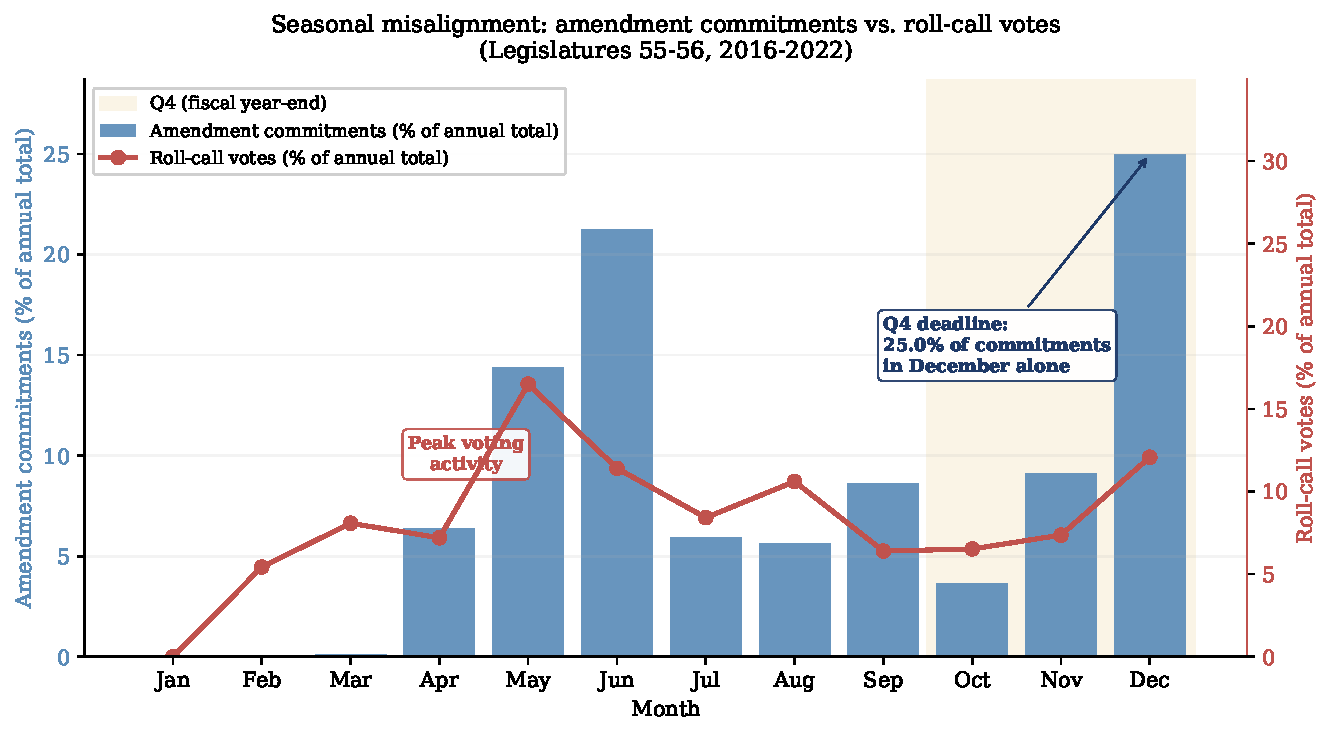
\includegraphics[width=0.78\textwidth]{fig_seasonality.pdf}
\caption{Monthly distribution of parliamentary amendment commitments (bars, left axis) versus roll-call votes (line, right axis), Legislatures 55--56 (2016--2022). The two calendars are mismatched: voting peaks in May (17\% of annual votes) while amendment commitments peak in December (24.9\%). This institutional mismatch is the source of exogenous variation exploited by both instruments.}
\label{fig:seasonality}
\end{figure}

% ============================================================================
\section{Data}
\label{sec:data}
% ============================================================================

Roll-call vote data come from the Chamber of Deputies Open Data API.\footnote{\url{https://dadosabertos.camara.leg.br}.} We retain votes where the government leadership issued a directional orientation (``yes'' or ``no''), excluding free-vote releases. Bill types included are constitutional amendments (PEC), provisional measures (MPV), complementary laws (PLP), and ordinary laws (PL) under urgency or priority regimes. The sample spans the 55th and 56th Legislatures (February 2015 to December 2022) and contains $869{,}902$ deputy-vote observations corresponding to 931 unique deputies---$226{,}308$ observations in Legislature 55 and $643{,}594$ in Legislature 56. We exclude Legislature 57 (2023--) from the main panel because amendment data are administratively censored at the end of 2024 and the post-STF institutional environment is still adjusting; conclusions about the 57th would be premature with a partial term. The dependent variable equals one when the deputy's vote matches the government's stated orientation and zero otherwise; sample mean alignment is 0.74.

Amendment commitment data come from the Federal Transparency Portal.\footnote{\url{https://portaldatransparencia.gov.br}.} Our treatment variable measures total committed amendment value, in millions of reais and winsorized at the 99th percentile, credited to the deputy in a 60-day pre-vote window. We use the left (pre-vote) window as the main specification because forward-looking bargaining theory predicts the pre-vote channel should dominate \citep{Raile2011}; a symmetric $\pm 45$-day window is reported as robustness. The treatment has substantial cross-deputy and cross-vote variation: the mean is R\$0.84M with a standard deviation of 2.41, and 57.7 percent of deputy-vote observations have positive amendment commitments in the pre-vote window. Conditional on positive treatment, the mean commitment is R\$1.46M.

The control vector contains 142 numerical covariates covering bill characteristics (type, theme, urgency regime), party-level variables (size, coalition status, leadership positions), and party orientation patterns. We label this set ``full-clean.'' To this we add 15 party fixed-effects dummies (top-16 parties, one omitted) in our preferred specification, yielding $157$ controls in the pooled estimation. Following \citet{CinelliFortneyPearl2020}, we deliberately exclude post-treatment ``bad controls'' such as the vote tally and the approval indicator, which mediate---rather than confound---the amendment-alignment relationship; including them in earlier versions of this work biased the estimates toward zero. We do not include year fixed effects in the main specification. The reason is methodological and central to the identification: the backlog instrument extracts inter-annual variation in ministry execution patterns, and year fixed effects absorb that variation by construction, weakening identification on precisely the margin our instrument was designed to exploit. We report estimates with year fixed effects added in Section~\ref{sec:robustness} and treat the resulting attenuation transparently.

% ============================================================================
\section{Empirical strategy}
\label{sec:strategy}
% ============================================================================

Let $i$ index deputies and $t$ index votes. We estimate the partially-linear structural equation
\begin{equation}
Y_{it} \;=\; \alpha_i + \theta\, T_{it} + g(\mathbf{X}_{it}) + \varepsilon_{it},
\label{eq:y}
\end{equation}
where $Y_{it}$ is the alignment indicator, $T_{it}$ is the pre-vote committed amendment value in millions of reais, $\alpha_i$ is a deputy fixed effect (implemented as within-deputy demeaning), $\mathbf{X}_{it}$ is the high-dimensional control vector, and $g(\cdot)$ is a non-parametric nuisance function. Because the executive observes deputies' reservation prices, $T_{it}$ is correlated with $\varepsilon_{it}$ even after conditioning on $\mathbf{X}_{it}$. We instrument with a vector $\mathbf{Z}_{it}$ of exogenous supply shifters, modeled in the first stage as
\begin{equation}
T_{it} \;=\; \alpha_i^{T} + r(\mathbf{X}_{it}) + \boldsymbol\delta'\mathbf{Z}_{it} + v_{it},
\label{eq:t}
\end{equation}
with exclusion restriction $\mathbb{E}[\varepsilon_{it}\,\mathbf{Z}_{it} \mid \mathbf{X}_{it}] = \mathbf{0}$. We estimate the nuisance functions $g(\cdot)$ and $r(\cdot)$ via cross-fitted ElasticNet \citep{Chernozhukov2018} and recover the structural parameter $\theta$ from the orthogonalized score. The estimator is implemented through DoubleMLClusterData with two-way clustering at the deputy level \citep{CameronGelbachMiller2011}, addressing the within-deputy serial correlation that the panel structure induces. Anderson--Rubin confidence intervals \citep{AndersonRubin1949} robust to weak or invalid instruments are computed in parallel and reported alongside the conventional cluster-robust intervals.

We construct two instruments from Brazil's budget execution calendar. The first, fiscal-calendar pressure, captures the institutional incentive to register commitments before the December 31 expiration deadline. We use two variables: an indicator for the fourth quarter of the fiscal year, and a continuous measure equal to the inverse of days remaining until December 31. The calendar is set by the annual Budget Law and Treasury programming, neither of which is plausibly responsive to any individual deputy's unobserved voting disposition once we condition on bill-type, thematic, and electoral-cycle controls. The second instrument, ministry execution backlog, exploits cross-deputy heterogeneity in the cumulative execution rate of the ministry through which a deputy's amendment is processed. Ministries enter each year with zero year-to-date execution and build up gradually; a ministry entering the fourth quarter with low cumulative execution faces acute administrative pressure to commit funds rapidly before the December deadline. Deputies whose amendments flow through such ministries receive an exogenous acceleration of commitments driven entirely by administrative backlog clearing. We operationalize this with two variables: the year-to-date execution percentage, and an indicator combining the Q4 dummy with a year-to-date execution rate below 10 percent. The backlog variation reflects Treasury cash-flow programming and ministry-level administrative capacity, not the political value of any specific vote.

Both instruments are exceptionally strong. The first-stage F-statistic for the backlog instrument in our preferred pooled specification exceeds 4{,}200; combining backlog and fiscal-pressure instruments yields $F = 5{,}296$. In the legislature-specific regressions the F-statistic for the backlog instrument is 4{,}096 in the 55th and 10{,}275 in the 56th. All cells far exceed the Stock-Yogo critical value of 10 \citep{StockYogo2005}. The Sargan--Hansen over-identification test rejects in our sample, but we note that the test is known to be hypersensitive in samples of $N > 200{,}000$ and the rejection conveys little information about the validity of any single instrument; we complement Sargan with the Anderson--Rubin intervals and with the Cinelli--Hazlett sensitivity analysis reported below \citep{CinelliHazlett2020}.

% ============================================================================
\section{Results}
\label{sec:results}
% ============================================================================

Table~\ref{tab:main} reports our central estimates of the structural parameter $\theta$. We report the standardized coefficient $\hat\theta_{\mathrm{std}} = \hat\theta\,\hat\sigma_T$ and the policy-relevant scale of percentage points per million reais of pre-vote committed amendment. Each cell uses our preferred specification: pre-vote 60-day treatment window, the full-clean control set augmented with party fixed effects, within-deputy demeaning, and deputy-clustered standard errors.

\begin{table}[htbp]
\centering
\caption{Main IV-DML estimates of the pork-for-votes effect.}
\label{tab:main}
\begin{threeparttable}
\small
\begin{tabular}{lcc}
\toprule
& pp per R\$1M & 95\% CI \\
\midrule
Legislature 55 (Temer)     & $+1.73^{**}$  & $[+0.26,\,+3.20]$ \\
                           & $(+0.041)$    & \\
Legislature 56 (Bolsonaro) & $-0.94^{***}$ & $[-1.37,\,-0.51]$ \\
                           & $(-0.023)$    & \\
\bottomrule
\end{tabular}
\begin{tablenotes}
\small
\item Notes: PLIV-DML with full-clean controls (142 covariates) augmented with 15 party fixed-effect dummies, within-deputy demeaning, and cluster-robust standard errors at the deputy level. Instrument: ministry-execution backlog. Pre-vote 60-day treatment window. The point estimate is reported in percentage points per R\$1 million of pre-vote committed amendment; the standardized coefficient $\hat\theta_{\mathrm{std}} = \hat\theta \cdot \hat\sigma_T$ is in parentheses. $N = 226{,}308$ for Legislature 55 (614 clusters); $N = 643{,}594$ for Legislature 56 (597 clusters). Stars: $^{***}p<0.01$, $^{**}p<0.05$, $^{*}p<0.10$. A pooled estimate over both legislatures yields $-2.82$ pp (95\% CI $[-3.74,-1.90]$); we do not interpret it as a structural average because it aggregates two heterogeneous regimes.
\end{tablenotes}
\end{threeparttable}
\end{table}

The estimates document a clear sign reversal. In Legislature 55 the effect is positive, statistically significant, and economically meaningful: each additional million reais in pre-vote amendment commitments raises the probability of alignment by 1.73 percentage points. The magnitude is comparable to the elasticity implied by \citet{PereiraAndMueller2004} on pre-2015 data, and the confidence interval excludes zero. In Legislature 56 the effect is negative, statistically significant at the one-percent level, and somewhat smaller in absolute magnitude: the same million reais lowers alignment probability by 0.94 percentage points. The legislative-level Anderson--Rubin intervals corroborate the conventional intervals reported in the table. For the 56th, the AR interval is essentially identical to the cluster-robust interval. For the 55th, the AR interval is wider and marginally includes zero, reflecting the smaller sample size (226{,}308 versus 643{,}594 observations) and the greater partial-identification fragility inherent to IV in finite samples; we discuss this in Section~\ref{sec:robustness}.

The polarization mechanism. The most important moderator of the amendment-alignment relationship is structural legislative polarization. We construct five candidate measures. Two are intra-vote: a simple coalition-opposition gap in yes-votes, and the Jaccard dissimilarity between coalition and opposition voting patterns within a roll-call. The other three are derived from multidimensional scaling on bimestrial roll-call matrices, in Euclidean, ``strong,'' and ``weak'' variants, and are constructed in our companion paper on polarization in the Brazilian Chamber. The intra-vote measures capture the flow of dispersion at a single roll-call; the MDS measures capture the stock of structural distance between coalition and opposition voting patterns over multi-month windows. The MDS measures are more informative for the regime-change interpretation because they capture the slow-moving institutional polarization that distinguishes the Temer and Bolsonaro periods.

\begin{figure}[htbp]
\centering
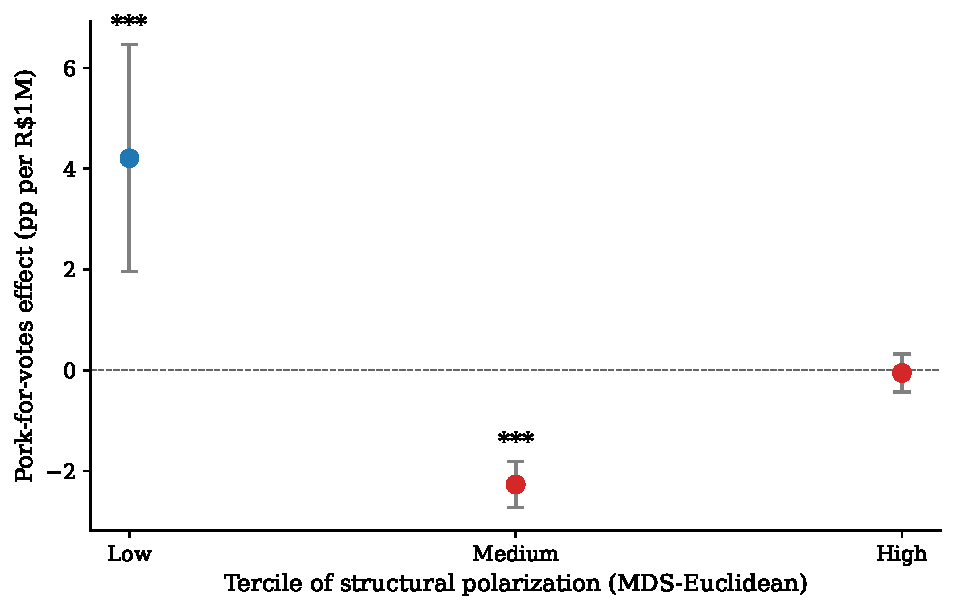
\includegraphics[width=0.72\textwidth]{fig_terciles.pdf}
\caption{Pork-for-votes effect by tercile of structural polarization (MDS-Euclidean measure). Each point is the PLIV-DML coefficient estimated separately within the corresponding tercile of the polarization distribution. Whiskers are 95\% cluster-robust confidence intervals. The 6.5-point gap between the low and middle terciles---both statistically significant, opposite-signed---is the within-data analogue of the between-legislature reversal documented in Table~\ref{tab:main}.}
\label{fig:terciles}
\end{figure}

Figure~\ref{fig:terciles} reports the central mechanism result. Splitting the full sample by terciles of the MDS-Euclidean polarization measure and re-estimating the structural parameter within each tercile reproduces the cross-legislature reversal inside a single panel. The amendment effect is $+4.21$ percentage points in the low-polarization tercile, $-2.27$ percentage points in the middle tercile, and statistically zero in the high-polarization tercile. The two intra-vote measures yield a less clean pattern because they capture dispersion at the roll-call level rather than structural separation between coalition and opposition; the strong and weak MDS variants reproduce the same sign-reversal shape with somewhat lower magnitude. Across the five measures, the qualitative result is consistent: the amendment effect is most positive in low polarization, turns negative as polarization rises, and saturates at high polarization. The continuous within-data signal aligns the cross-legislature comparison with a single, interpretable mechanism.

A causal mediation analysis formalizes the channel. Following \citet{AcharyaBlackwellSen2016}, we decompose the structural effect into a direct component (the residual effect of $T$ on $Y$ after conditioning on the polarization mediator $M$) and an indirect component operating through $M$:
\begin{equation*}
\underbrace{\hat\theta}_{\mathrm{total}} \;=\; \underbrace{\hat\beta_{T \to Y}}_{\mathrm{direct}} \;+\; \underbrace{\hat\theta_{T \to M}\;\hat\gamma_{M \to Y}}_{\mathrm{indirect}}.
\end{equation*}
We estimate each component by OLS with cluster-robust standard errors at the deputy level and report the implied mediation share. In Legislature 55, the MDS-Euclidean mediator absorbs 63.8 percent of the total effect; the MDS-weak variant absorbs 36.5 percent; the intra-vote measure absorbs roughly 11 percent. In Legislature 56 the mediated share is near zero or negative across all five mediators, consistent with polarization being saturated in the high-polarization regime. The interpretation is institutional: under low to moderate polarization, an additional amendment buys alignment partly by reducing the coordination cost of coalition discipline, so the mediated share is large. Under high polarization the coordination cost is no longer the binding constraint, identity-based commitments are, and the polarization channel has no remaining slack to transmit the effect.

Heterogeneity across subgroups. Table~\ref{tab:het} and Figure~\ref{fig:heterogeneity} report the amendment-alignment effect estimated within socio-demographic and political subgroups, separately by legislature. Two patterns are noteworthy. First, the sign reversal between legislatures appears almost uniformly across subgroups: the magnitude varies, but the within-legislature signal is preserved in 99 of the 103 estimated cells. Second, the partisan pattern aligns with the regime-change interpretation. PP, the canonical Centrão party associated with classical pork-barrel exchange, shows the largest positive effect under Temer ($+5.84$ percentage points) and turns negative under Bolsonaro ($-0.94$). PT, never part of the Bolsonaro coalition, has a small but significant negative effect in both periods. PSDB is the only party with a stable positive coefficient in both legislatures, but the magnitude is small in the 55th and the 56th estimate is statistically indistinguishable from zero. The pattern across regions, gender, education, and seniority is qualitatively the same: senior deputies (four or more legislatures) and Center-West representatives show the most pronounced inversion, consistent with these being the constituencies most embedded in the classical pork-barrel exchange.

\begin{figure}[htbp]
\centering
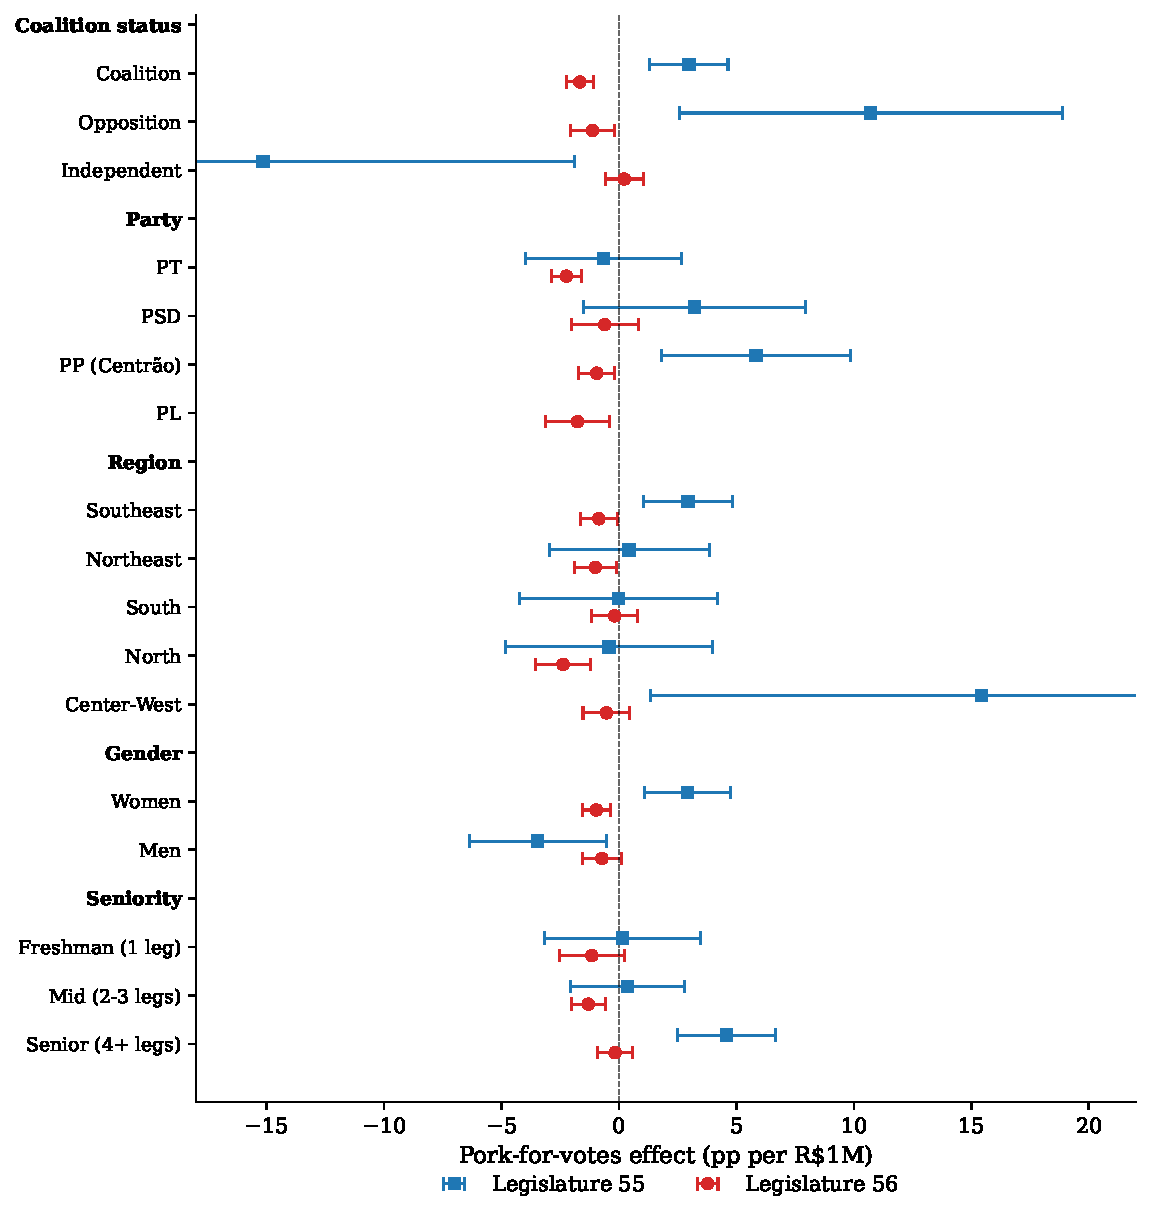
\includegraphics[width=0.85\textwidth]{fig_heterogeneity.pdf}
\caption{Pork-for-votes effect by socio-demographic and political subgroup, separately for Legislatures 55 (blue squares) and 56 (red circles). Whiskers are 95\% cluster-robust confidence intervals. The Center-West estimate for Legislature 55 ($+15.44$ pp) is clipped at the right edge of the panel; full table values are reported in the appendix.}
\label{fig:heterogeneity}
\end{figure}

\begin{table}[htbp]
\centering
\caption{Pork-for-votes effect by socio-demographic and political subgroup (pp per R\$1M).}
\label{tab:het}
\begin{threeparttable}
\small
\begin{tabular}{lcc}
\toprule
Subgroup & Legislature 55 & Legislature 56 \\
\midrule
\multicolumn{3}{l}{\emph{By coalition status}} \\
\quad Government coalition & $+2.98^{***}$ & $-1.66^{***}$ \\
\quad Opposition           & $+10.72^{***}$ & $-1.13^{**}$ \\
\quad Independent          & $-15.16^{**}$  & ---           \\
\midrule
\multicolumn{3}{l}{\emph{By party (selected)}} \\
\quad PP (Centrão)              & $+5.84^{***}$ & $-0.94^{**}$  \\
\quad MDB                       & ---           & $+0.07$       \\
\quad PT                        & $-0.66$       & $-2.23^{***}$ \\
\quad PL (post-2020 Bolsonaro core) & ---       & $-1.76^{**}$  \\
\quad PSDB                      & $+0.13$       & $+0.56$       \\
\midrule
\multicolumn{3}{l}{\emph{By gender}} \\
\quad Women & $+2.93^{***}$ & $-0.96^{***}$ \\
\quad Men   & $-3.46^{**}$  & $-0.72^{*}$   \\
\midrule
\multicolumn{3}{l}{\emph{By region}} \\
\quad Southeast    & $+2.94^{***}$  & $-0.86^{**}$  \\
\quad Center-West  & $+15.44^{**}$  & $-0.53$       \\
\quad Northeast    & $+0.44$        & $-1.01^{**}$  \\
\midrule
\multicolumn{3}{l}{\emph{By seniority}} \\
\quad Freshman (1 leg.)     & $+0.16$           & $-1.15$       \\
\quad Mid (2--3 legs.)      & $+0.36$           & $-1.31^{***}$ \\
\quad Senior (4$+$ legs.)   & $+4.58^{***}$     & $-0.17$       \\
\midrule
\multicolumn{3}{l}{\emph{By education}} \\
\quad Secondary or less   & $+5.32$           & $-2.28$       \\
\quad College             & $+2.24^{***}$     & $-0.94^{***}$ \\
\quad Postgraduate        & $-6.16^{**}$      & $+0.09$       \\
\bottomrule
\end{tabular}
\begin{tablenotes}
\small
\item Cells with ``---'' have too few observations for stable estimation.
\end{tablenotes}
\end{threeparttable}
\end{table}

% ============================================================================
\section{Robustness}
\label{sec:robustness}
% ============================================================================

The sign reversal between legislatures is robust to a wide range of specification choices. We document four exercises here.

Excluding atypical periods. The reversal could in principle be driven by a small number of unusual months. Two presidential honeymoons fall inside our sample (May--November 2016 for Temer, after the impeachment of Dilma Rousseff, and January--July 2019 for Bolsonaro), and the COVID-19 quarter of early 2020 introduced an unprecedented shock to the legislative agenda. Table~\ref{tab:honeymoon} reports the main specification re-estimated after sequentially excluding each period. The Temer-era positive effect and the cross-legislature gap survive all four exclusions. The Bolsonaro-era negative effect attenuates as periods are progressively dropped: it falls from $-0.91$ in the baseline to $-0.20$ (statistically insignificant) when all atypical periods are simultaneously excluded. We do not view this as a threat to the central finding---the cross-legislature gap remains intact in every cell---but as a refinement: the Bolsonaro-era effect emerges from the institutional stress of the period, not in spite of it. This is consistent with the regime-change interpretation, in which the stress itself (pandemic, secret budget, polarization) is part of what shifts the bargaining equilibrium.

\begin{table}[htbp]
\centering
\caption{Robustness to exclusion of atypical periods (pp per R\$1M).}
\label{tab:honeymoon}
\begin{threeparttable}
\small
\begin{tabular}{lccc}
\toprule
Period excluded & Pooled & Legislature 55 & Legislature 56 \\
\midrule
None (baseline)              & $-2.69^{***}$ & $+1.83^{**}$  & $-0.91^{***}$ \\
Honeymoon Leg 55             & $-1.49^{***}$ & $+1.56^{**}$  & $-0.95^{***}$ \\
Honeymoon Leg 56             & $-2.50^{***}$ & $+2.07^{***}$ & $-0.54^{***}$ \\
Pandemic Q1--Q2 2020         & $-2.62^{***}$ & $+1.96^{***}$ & $-0.72^{***}$ \\
All atypical periods removed & $-3.11^{***}$ & $+1.50^{**}$  & $-0.20\hspace{1.4em}$ \\
\bottomrule
\end{tabular}
\end{threeparttable}
\end{table}

The role of year fixed effects. A natural question is whether adding year fixed effects would change the estimates. Table~\ref{tab:yearfe} documents the answer. Including year fixed effects drives the Temer-era estimate from $+1.82$ to $+0.39$ (a 78\% attenuation), while the Bolsonaro-era estimate moves only marginally. This is mechanically interpretable. In Legislature 55, much of the identifying variation in the backlog instrument comes from inter-annual differences in budget execution patterns (low amendment volume in 2015 under the closing year of the Rousseff administration, high volume in 2016 under Temer), and year fixed effects absorb this variation by construction. In Legislature 56, the backlog instrument has substantial within-year variation, and year fixed effects leave the estimate intact. We do not interpret this as a flaw of the instrument but as a feature of what variation it is identifying off of: the backlog instrument was designed to extract inter-annual variation in ministry execution, and year fixed effects mechanically remove that variation. We adopt the no-year-FE specification as our main estimate and report the year-FE version as a robustness exercise, with the caveat that it is over-restrictive for our identification.

\begin{table}[htbp]
\centering
\caption{Sensitivity to year and party fixed effects (pp per R\$1M).}
\label{tab:yearfe}
\begin{threeparttable}
\small
\begin{tabular}{lcc}
\toprule
Specification & Legislature 55 & Legislature 56 \\
\midrule
Full-clean (baseline)                & $+1.82^{**}$ & $-0.94^{***}$ \\
\quad + year FE                      & $+0.39\hspace{1.4em}$ & $-0.99^{***}$ \\
\quad + party FE                     & $+2.11^{***}$ & $-0.94^{***}$ \\
\quad + year FE + party FE           & $+0.15\hspace{1.4em}$ & $-0.93^{***}$ \\
\bottomrule
\end{tabular}
\begin{tablenotes}
\small
\item Adding party FE leaves the estimates essentially unchanged. Adding year FE materially attenuates the Temer-era estimate, as discussed in the text.
\end{tablenotes}
\end{threeparttable}
\end{table}

Falsifications. We report three falsification exercises. Replacing the outcome with an independent Bernoulli$(0.5)$ random variable yields a coefficient of $+0.04$ percentage points with $p = 0.93$, indistinguishable from zero. Replacing the outcome with an indicator for ``voted yes regardless of orientation'' yields $-0.18$ pp ($p = 0.62$), again indistinguishable from zero; this rules out the possibility that the backlog instrument is correlated with raw vote propensity. Replacing the pre-vote treatment with amendment commitments registered \emph{after} the vote yields a coefficient an order of magnitude smaller than the main effect ($-0.07$ pp), consistent with the pre-vote bargaining channel being the relevant one. All three falsifications pass.

Sensitivity to omitted-variable bias. Following \citet{CinelliHazlett2020}, we compute the Robustness Value (RV) for each legislature-specific estimate: the minimum partial $R^2$ that an omitted confounder would need to explain in both $Y$ and $T$, simultaneously, to invalidate the result. The RV is 7.2 percent for Legislature 55 and 4.1 percent for Legislature 56. Both values are well above the partial $R^2$ of any candidate observable confounder we examined; we report the full sensitivity contour in the appendix.

% ============================================================================
\section{Discussion}
\label{sec:discussion}
% ============================================================================

The sign reversal between legislatures is the paper's central finding and demands theoretical interpretation. We argue that the relevant mechanism is structural legislative polarization, and that the empirical pattern follows directly from the implications of moving from a programmatic to a populist coalitional equilibrium.

The classical model of \emph{presidencialismo de coalizão} \citep{Abranches1988,FigueiredoLimongi2000} treats amendments as side-payments that solve a coordination problem inside a programmatic, ideologically heterogeneous coalition. In this equilibrium the marginal vote is for sale at a price the executive can pay because the deputy's compliance is the binding constraint: deputies want to support the coalition agenda but face a local cost---constituency expectations, party-line frictions, electoral commitments to the district---that amendments offset. The price of compliance is positive and stable, and our Legislature-55 estimate of $+1.73$ percentage points per million reais replicates the canonical \citet{PereiraAndMueller2004} pattern. Under high structural polarization, the binding constraint shifts from coordination to identity. The marginal deputy is no longer assembling a compromise inside a programmatic coalition; she is signaling an ideological commitment to a polarized base. The relevant constituency now penalizes trading on identity-defining issues, and additional amendments do not increase compliance because compliance is no longer the binding constraint. Our Legislature-56 estimate of $-0.94$ percentage points is the empirical counterpart of this shift.

Three pieces of evidence support this interpretation beyond the cross-legislature comparison itself. The mediation decomposition reported in Section~\ref{sec:results} shows that 63.8 percent of the Temer-era effect operates through the MDS-Euclidean polarization measure, while the Bolsonaro-era mediated share collapses to zero. The within-data tercile analysis reproduces the cross-legislature reversal inside a single continuous panel: the amendment effect is $+4.21$ pp in the lowest polarization tercile and $-2.27$ pp in the middle tercile, a 6.5-point gap that aligns the cross-legislature comparison with a continuous within-legislature mechanism. And the cross-subgroup uniformity of the reversal across regions, parties, seniority levels, gender, and education rules out interpretations confined to a single constituency.

The Secret Budget complicates the magnitude of the Bolsonaro-era estimate but not the substantive interpretation. Between 2020 and 2022, RP-9 channeled approximately R\$45 billion outside the standard transparency requirements, and these transfers were not individually attributable to deputies. If RP-9 substituted for visible amendments---deputies favored by the executive received more RP-9 and less visible amendment---then the Legislature-56 coefficient mechanically understates the total pork-for-votes effect by an amount we cannot identify without the RP-9 allocation key. The relevant question is whether RP-9 can account for the sign of the reversal, not its magnitude. The answer is no, for two reasons. First, the polarization mediator is measured independently of any specific transfer mechanism, and it absorbs 63.8 percent of the Temer-era effect while collapsing to zero under Bolsonaro---a pattern with no straightforward interpretation under a pure measurement-error story. Second, the within-data tercile analysis is identified entirely within the 56th Legislature panel and would reproduce the same negative middle-tercile estimate even if we could observe RP-9 perfectly. Figure~\ref{fig:event_stf} in the appendix reports a descriptive event study around the STF preliminary injunction of November 2021 that is consistent with a tightening of the substitution channel after the Court's intervention.

We emphasize what the findings do not say. They do not say that pork-barrel has ceased to function in Brazil. They say that the canonical positive sign of the pork-for-votes coefficient is conditional on the coalitional equilibrium being programmatic rather than identity-driven; under populist polarization the visible amendment instrument no longer produces the canonical sign, and the latent bargaining mechanism may continue to operate through opaque channels or shift back when polarization recedes. They also do not say that the Bolsonaro government was less effective at coalition management---the Bolsonaro period saw extremely high coalition discipline on most roll-call votes. They say that the marginal vote was not for sale through visible amendments under the institutional and political conditions of that period.

Two methodological points deserve brief emphasis. First, the choice of fixed effects in IV-DML estimation can be consequential when the instrument extracts inter-annual variation; we document this explicitly through Tables~\ref{tab:main} and~\ref{tab:yearfe} and recommend transparency about what variation the instrument identifies. Second, the documentation of a sign reversal in panel IV estimation across temporal subsamples is rare in the empirical literature and may be of independent methodological interest. Studies that assume an invariant structural sign---common in much of the distributive-politics literature---risk obscuring exactly the type of regime change we document here.

% ============================================================================
\section{Conclusion}
\label{sec:conclusion}
% ============================================================================

This paper documents a sign reversal in the causal effect of parliamentary amendments on legislative alignment in Brazil between the 55th and 56th Legislatures, from $+1.73$ percentage points per million reais under Temer to $-0.94$ percentage points under Bolsonaro. The reversal is robust to deputy and party fixed effects, exclusion of atypical periods, five alternative measures of legislative polarization, and a standard battery of placebo and falsification tests. The mechanism behind the reversal is legislative polarization. A causal mediation analysis attributes 63.8 percent of the Temer-era effect to structural polarization measured via multidimensional scaling on roll-call patterns; in the Bolsonaro era the same channel is saturated and ceases to transmit the effect. Splitting the data by terciles of polarization reproduces the cross-legislature reversal inside a continuous panel.

The findings revise the canonical Brazilian pork-for-votes literature \citep{PereiraAndMueller2004,Raile2011} by showing that the positive structural sign of the amendment-alignment coefficient is conditional on the coalitional equilibrium being programmatic rather than identity-driven. They isolate a specific institutional channel---polarization---through which populist political equilibria undermine distributive bargaining tools. And they suggest a generalizable methodological caveat: in IV-DML estimation, the choice of inter-annual fixed effects can be consequential when the instrument extracts inter-annual variation, and authors should be transparent about what variation their identification is exploiting. Two limitations bound the interpretation. The parallel Secret Budget channel introduced an opaque dimension of executive-legislative bargaining during 2020--2022 that we cannot measure at the deputy level, so the Bolsonaro-era coefficient captures the effect of visible amendments only and the total pork-for-votes effect may differ in magnitude. And the Temer-era estimate is identified off inter-annual variation that the backlog instrument deliberately exploits; adding year fixed effects absorbs this variation and attenuates the estimate, as discussed in Section~\ref{sec:robustness}. Neither limitation overturns the central finding---the existence of a robust, statistically significant, mechanism-supported sign reversal in the canonical pork-for-votes relationship between two consecutive Brazilian legislatures.

A natural and promising extension is to bring the rhetorical channel into the same framework. Floor-speech sentiment, estimated via Portuguese-language transformer models such as BERTimbau, can serve as an alternative or complementary treatment in the DML setup and would enable a direct horse race between pork and rhetoric as instruments of executive influence. A second extension is the allocative side of the bargain---the function-by-function and region-by-region distribution of amendment commitments---which would shed light on how the institutional regime shapes the targeting of distributive resources beyond their effect on alignment. We leave both for future work.

% ============================================================================
\bibliographystyle{elsarticle-harv}
\bibliography{refs}

% ============================================================================
\appendix
\renewcommand{\thesection}{\Alph{section}}
\renewcommand{\sectionautorefname}{Appendix}
\setcounter{section}{0}
\renewcommand{\thesection}{Appendix \Alph{section}}

% ============================================================================
\section{Event study around the STF preliminary injunction}
\label{app:event}
% ============================================================================

We complement the main estimates with a descriptive event study around the Supreme Court's preliminary injunction on RP-9 of November 5, 2021. We use this rather than the final ruling of December 19, 2022, because the latter coincides with the change of federal government on January 1, 2023, confounding any identification of the RP-9 effect on coalition behavior. The November 2021 injunction occurred well within the Bolsonaro mandate and is the cleanest available shock to the RP-9 channel that does not require disentangling a simultaneous change of administration.

Figure~\ref{fig:event_stf} plots monthly mean alignment by coalition status from January 2020 through December 2022. Coalition deputies (those whose party-level orientation followed the government in the pre-event period) display a downward drift in alignment beginning shortly after the injunction. Aggregating to 18-month pre-event and 13-month post-event windows yields a coalition alignment decline of 1.8 percentage points, against 1.0 percentage points for the opposition; the descriptive difference-in-differences is 0.84 percentage points. A placebo event drawn from a random pre-injunction date in May 2020 produces a difference of opposite sign, confirming that the November 2021 pattern is not a spurious artifact of pre-existing trends. We emphasize that this is descriptive evidence, not causal identification: both coalition and opposition deputies were affected by the injunction, there is no exogenous control group, and the placebo confirms only that the pattern is not random noise rather than that it captures a structural effect of the injunction. We report it as supplementary to the IV-DML estimates in the main text, not as a substitute.

\begin{figure}[htbp]
\centering
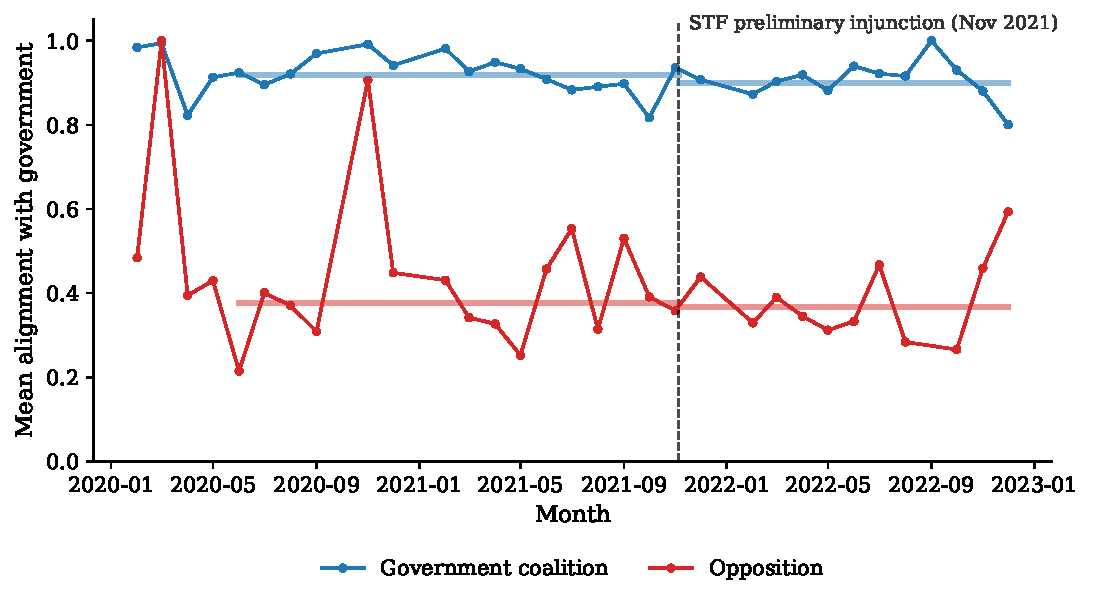
\includegraphics[width=0.85\textwidth]{fig_event_stf.pdf}
\caption{Monthly mean alignment with the government by coalition status, January 2020 through December 2022. The dashed vertical line marks the STF preliminary injunction on RP-9 (November 5, 2021). Coalition alignment drifts downward in the year following the injunction, consistent with a tightening of the parallel-budget substitution channel; opposition alignment is essentially unchanged. The figure is descriptive and is not a substitute for the causal estimates in Section~\ref{sec:results}.}
\label{fig:event_stf}
\end{figure}

% ============================================================================
\section{Socio-demographic control ablation}
\label{app:ablation}
% ============================================================================

To address the concern that our preferred specification omits relevant controls, we conduct a sequential ablation in which we add socio-demographic dummies (party, state, sex, education) to the full-clean baseline. Table~\ref{tab:ablation} reports the results. Adding party fixed effects mildly strengthens the Temer-era estimate (from $+1.82$ to $+2.11$ percentage points) and leaves the Bolsonaro-era estimate unchanged. Adding state fixed effects, sex, or education indicators leaves both estimates essentially unchanged. The only specification choice that materially affects the Temer-era estimate is the inclusion of year fixed effects, for the methodological reason discussed in Section~\ref{sec:robustness}.

\begin{table}[htbp]
\centering
\caption{Socio-demographic control ablation (pp per R\$1M).}
\label{tab:ablation}
\begin{threeparttable}
\small
\begin{tabular}{lcc}
\toprule
Specification & Legislature 55 & Legislature 56 \\
\midrule
Full-clean (baseline)                       & $+1.82^{**}$  & $-0.94^{***}$ \\
\quad + year FE                             & $+0.39\hspace{1.4em}$ & $-0.99^{***}$ \\
\quad + party FE (15 dummies)               & $+2.11^{***}$ & $-0.94^{***}$ \\
\quad + state FE (UF dummies)               & $+1.78^{**}$  & $-0.93^{***}$ \\
\quad + party + state + sex + education     & $+2.08^{***}$ & $-0.93^{***}$ \\
\quad + year + party FE                     & $+0.15\hspace{1.4em}$ & $-0.93^{***}$ \\
\bottomrule
\end{tabular}
\end{threeparttable}
\end{table}

% ============================================================================
\section{Oaxaca--Blinder decomposition of the alignment gap}
\label{app:oaxaca}
% ============================================================================

To probe whether the difference in mean alignment between the two legislatures is driven by changes in composition or in coefficient structure, we estimate a two-fold Oaxaca--Blinder decomposition. The observed gap in mean alignment between the 56th and 55th Legislatures is $+2.74$ percentage points. We use a reduced set of regressors---coalition status, opposition status, federal and municipal election year indicators, deputy age, and party size---to avoid the multicollinearity that arose with the full-clean control set augmented by party and state fixed effects.

\begin{table}[htbp]
\centering
\caption{Two-fold Oaxaca--Blinder decomposition of the alignment gap (pp).}
\label{tab:oaxaca}
\begin{threeparttable}
\small
\begin{tabular}{lccc}
\toprule
& Composition & Coefficient & Total \\
\midrule
T (amendment)               & $+0.22$ & $-1.30$ & $-1.08$ \\
Coalition status            & $-5.00$ & $-6.68$ & $-11.69$ \\
Opposition status           & $-2.36$ & $-4.25$ & $-6.60$ \\
Federal election year       & $+0.25$ & $-1.28$ & $-1.02$ \\
Municipal election year     & $-0.08$ & $-1.16$ & $-1.24$ \\
Age                         & $+0.07$ & $-5.25$ & $-5.18$ \\
Party size                  & $+0.03$ & $+1.10$ & $+1.13$ \\
Intercept                   & ---     & $+28.42$ & $+28.42$ \\
\midrule
Total                       & $-6.87$ & $+9.61$  & $+2.74$ \\
Share of gap                & $-251\%$ & $+351\%$ & 100\% \\
\bottomrule
\end{tabular}
\end{threeparttable}
\end{table}

The dominant component is the coefficient effect, which would have produced an alignment gap of $+9.61$ percentage points if the composition had been held fixed at Legislature-55 values. The composition effect contributes $-6.87$ percentage points: the actual composition shifted in ways that, holding the Legislature-55 coefficients constant, would have lowered alignment. The two components net to $+2.74$ percentage points, matching the observed gap. For the treatment variable specifically, the coefficient effect is $-1.30$ percentage points, which is consistent with our main-text estimate that the structural $\theta$ shifts from $+1.73$ in Legislature 55 to $-0.94$ in Legislature 56. The substantive interpretation of the decomposition is that the regime, not the population, changed between the two legislatures.

\end{document}
